\begin{enumerate}
  \item 
\begin{enumerate}
  \item Dans l'intervalle considéré, $\sin \frac{\alpha}{2}$ et $\tan \alpha$ sont strictement positives. Pour les comparer, il est bien plus commode de les diviser que de les soustraire.
\begin{displaymath}
\forall \alpha \in I,\hspace{0.5cm} \frac{2\sin(\frac{\alpha}{2})}{\tan(\alpha)} = \frac{2\sin \frac{\alpha}{2}\cos \alpha}{\sin \alpha}
= \frac{\cos \alpha}{\cos \frac{\alpha}{2}} < 1
\end{displaymath}
car $\frac{\alpha}{2} < \alpha$ et $\cos$ décroissante dans $I$.

  \item Le calcul est habituel (avec $\sin\frac{\alpha}{2}>0$ car $0<\frac{\alpha}{2}<\frac{\pi}{4}$):
\begin{displaymath}
  e^{i\alpha} -1 = e^{i\frac{\alpha}{2}}(e^{i\frac{\alpha}{2}}-e^{-i\frac{\alpha}{2}})=2ie^{i\frac{\alpha}{2}}\sin\frac{\alpha}{2}
  \Rightarrow \left|e^{i\alpha} -1\right| = 2 \sin\frac{\alpha}{2} 
\end{displaymath}
Le complexe $z$ est de la forme $\lambda e^{i\alpha}$ avec $\lambda\in \R$ et $\Re(z)=1$. On obtient
\begin{displaymath}
  \lambda \cos \alpha = 1 \;\Rightarrow\; z = \frac{1}{\cos \alpha}e^{i\alpha}
\end{displaymath}
D'après les calculs précédents, sur la figure \ref{fig:Cgregory_1}, la longueur $2\sin(\frac{\alpha}{2})$ du segment de corde est inférieure à $\tan(\alpha)$ qui est la longueur du segment de tangente.

\end{enumerate}
\begin{figure}[h]
  \centering
  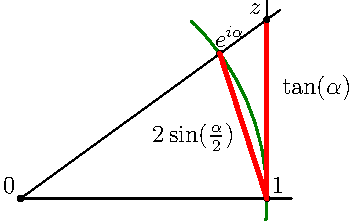
\includegraphics{./Cgregory_1.pdf}
  % Cgregory_1.pdf: 0x0 pixel, 0dpi, 0.00x0.00 cm, bb=
  \caption{Interprétation géométrique de l'inégalité.}
  \label{fig:Cgregory_1}
\end{figure}

  \item La longueur d'un segment utilisé dans l'approximation est un module du type calculé en 1.b. D'une étape à l'autre, l'angle est divisé par $2$ et le nombre de segment double  : $1=2^0, 2=2^1, 4=2^2, \cdots$. On en tire
\begin{multline*}
  e_0 = 2\sin\frac{\pi}{2^3},\; e_1 = 2\times(2\sin\frac{\pi}{2^4})=2^2\sin\frac{\pi}{2^4},\;
  e_2 = 2^2\times(2\sin\frac{\pi}{2^5}) = 2^3\sin\frac{\pi}{2^5},\\
  \;\cdots\;,\;
  c_n = 2^n\times(2\sin\frac{\pi}{2^{n+3}}) = 2^{n+1}\sin\frac{\pi}{2^{n+3}} \; 
  \Rightarrow \; e_n = 2^{n+1}\sin\frac{\pi}{2^{n+3}}
\end{multline*}
On peut remarquer que $a_n = \frac{\pi}{4}a(\frac{\pi}{2^{n+3}})$. 
  \item Si $0 < \theta < \frac{\pi}{4}$ alors $0 < 2\theta < \frac{\pi}{2}$ donc $\sin \theta$ et $\cos \theta$ sont strictement positifs.
\begin{displaymath}
  \frac{1}{\tan 2\theta} + \frac{1}{\sin 2\theta}
=\frac{\cos 2\theta + 1}{\sin 2\theta} = \frac{2\cos^2 \theta -1 + 1}{2\sin \theta \, \cos \theta} = \frac{1}{\tan \theta}
\end{displaymath}
\begin{displaymath}
  \frac{(\sin 2\theta)(\tan \theta)}{2} = \frac{2\sin \theta \cos \theta \sin \theta}{2 \cos \theta} = \sin^2 \theta
\Rightarrow
\sqrt{\frac{(\sin 2\theta)(\tan \theta)}{2}}= \sin \theta
\end{displaymath}

  \item
\begin{enumerate}
  \item Notons $\theta = \frac{\alpha}{2^{n+1}}$, alors $\frac{\alpha}{2^n}=2\theta$. Multiplions par $2\theta$ la première relation obtenue à la question 3. et introduisons $a$ et $b$. On obtient
\begin{displaymath}
2a(\theta) = b(2\theta) + a(2\theta)\Leftrightarrow a_{n+1} = a(\theta) = \frac{1}{2}\left(a(2\theta) + b(2\theta) \right)=\frac{1}{2}(a_n + b_n)   
\end{displaymath}
De manière analogue, en divisant la deuxième relation par $\theta$,
\begin{displaymath}
\frac{1}{b(\theta)} = \frac{1}{\sqrt{b(2\theta)a(\theta)}}\Leftrightarrow b_{n+1} = \sqrt{b_n\,a_{n+1}}  
\end{displaymath}

  \item Si on initialise la récurrence de Gregory avec $\alpha = \frac{\pi}{4}$ c'est à dire
\begin{displaymath}
a_0 = \frac{\alpha}{\tan \alpha } = \alpha \text{ et }   b_0 = \frac{\alpha}{\sin \alpha } = \sqrt{2} \alpha
\end{displaymath}
On obtient deux suites qui convergent vers $1$. Cela n'a pas l'air très utile pour un calcul numérique de $\pi$ puisqu'il apparait dans l'initialisation alors l'objectif est justement de l'évaluer. L'intérêt vient du caractère \emph{homogène} des relations. Si pour une suite vérifiant la relation de Gregory, on multiplie les deux conditions initiales par un \emph{même} $\lambda >0$, alors la proportionnalité se propage. On en déduit que les suites vérifiant les relations de Gregory avec les conditions initiales $1$ et $\sqrt{2}$ sont 
\begin{displaymath}
  \frac{4}{\pi}a(\frac{\alpha}{2^n}) \text{ et } \frac{4}{\pi}b(\frac{\alpha}{2^n})
\end{displaymath}
Elles sont assez commodes à calculer numériquement à cause de la simplicité des relations de récurence et elles convergent vers $\frac{4}{\pi}$.
\end{enumerate}

\item
\begin{enumerate}
  \item Pour $x$ non nul,
\begin{multline*}
  \frac{1}{\th(2x)} = \frac{e^{2x} + e^{-2x}}{e^{2x} - e^{-2x}}
  = \frac{(e^{x} + e^{-x})^2-1}{(e^{x} - e^{-x})(e^{x} + e^{-x})} \\
  = \frac{e^{x} + e^{-x}}{(e^{x} - e^{-x}} - \frac{-1}{(e^{x} - e^{-x})(e^{x} + e^{-x})}
  = \frac{1}{\th x} - \frac{1}{\sh x}
\end{multline*}
La première formule est donc exactement analogue:
\begin{displaymath}
  \frac{1}{\th x} = \frac{1}{\th(2x)} + \frac{1}{\sh(2x)}
\end{displaymath}
D'autre part:
\begin{displaymath}
\frac{1}{2}\sh(2x) \th x = \frac{1}{4}(e^{x}+e^{-x}) (e^{x}-e^{-x})\frac{(e^{x}-e^{-x})}{(e^{x}+e^{-x})} = (\sh x)^2 
\end{displaymath}
La deuxième formule est aussi exactement analogue pour les $x>0$:
\begin{displaymath}
  \sh x = \sqrt{\frac{(\sh(2x))(\sh x)}{2}}
\end{displaymath}

  \item Par définition de $\th$ et $\sh$, comme $e^{\ln 2} = 2$,
\begin{displaymath}
\th(\ln(2)) = \frac{2-\frac{1}{2}}{2+\frac{1}{2}} = \frac{3}{5},\hspace{0.5cm}
\sh(\ln(2)) = \frac{2-\frac{1}{2}}{2} = \frac{3}{4}
\end{displaymath}

  \item Notons $\alpha = \ln(2)$, et notons encore $a$ et $b$ les versions hyperboliques des fonctions définies au début de l'énoncé. Alors 
\begin{displaymath}
\left\lbrace 
\begin{aligned}
a(\alpha) &= \frac{5}{3}\ln 2 = 5 \times \frac{\ln 2}{3}\\
b(\alpha) &= \frac{4}{3}\ln 2 = 4 \times \frac{\ln 2}{3} 
\end{aligned}
\right. 
\end{displaymath}
On remarque que cette fois $a(x)>b(x)$ pour $x>0$.\newline
Par un raisonnement analogue à celui de la question 4.a., les suites des $a(\frac{\alpha}{2^n})$ et  $b(\frac{\alpha}{2^n})$ vérifient les relations de récurrence de Gregory avec les conditions initiales $\frac{5}{3}\ln 2$ et $\frac{4}{3}\ln 2$.\newline
Si on multiplie ces deux conditions initiales par un même réel $\lambda >0$, les relations de récurrence vont propager cette proportionalité et toutes les valeurs des suites seront multipliées par $\lambda$. On en déduit que, pour les suite de l'énoncé,
\begin{displaymath}
\forall n \in \N,\hspace{0.5cm} a_n = \frac{3}{\ln 2}a(\frac{\ln 2}{2^n}),\hspace{0.5cm}  b_n = \frac{3}{\ln 2}b(\frac{\ln 2}{2^n})
\end{displaymath}
On en déduit que les deux suites convergent vers $\frac{3}{\ln 2}$.
\end{enumerate}
\end{enumerate}
